\documentclass[msc,oneside]{ubcthesis}%msc, phd, masc, ma, or meng

% ================================================================================
% CHANGE THE FOLLOWING ACCORDING TO YOUR PROGRAM/THESIS
% ================================================================================
\institution{The University Of British Columbia}
\faculty{Unit 5}
\institutionaddress{Okanagan}

% For an Honours thesis, use \documentclasss[msc,oneside]{ubcthesis} above and
% uncomment and modify the next line:
\degreetitle{B.Sc. Computer Science Honours}

\title{Honours Computer Science Thesis}
\subtitle{\emph{rally}, a one stop-shop for all reddit data}
\author{Kevin J. Eger}
\copyrightyear{2016}
\submitdate{April 2016} % date of approved thesis
\program{Computer Science}%or Mathematics, or Interdisciplinary Studies

% ================================================================================


\usepackage{ubcostyle} %loads packages


% ===================================================================
% CHANGE THE FOLLOWING COMMANDS ACCORDING TO YOUR NEEDS
% ===================================================================
\newcommand{\R}{\mathbb{R}}   %real number
\newcommand{\Z}{\mathbb{Z}}   %integers
\newcommand{\C}{\mathbb{C}}   %complex numbers

\newcommand{\dom}{\operatorname{dom}}
\providecommand{\TT}[1]{\Theta\left(#1\right)} % big-Theta
\providecommand{\OO}[1]{\mathcal{O}\left(#1\right)} % big-Oh
\setlength{\parskip}{1em}
% ===================================================================

%Uncomment the next line if there are more than one appendix
%\renewcommand*\appendixname{Appendices}

\usepackage{graphicx}
\graphicspath{ {images/} }
\usepackage[section]{placeins}

\usepackage{xcolor}
\usepackage{listings}
\usepackage[T1]{fontenc}

\lstset{	
	language=PHP,
    breaklines=true,
    postbreak=\raisebox{0ex}[0ex][0ex]{\ensuremath{\color{red}\hookrightarrow\space}},
    tabsize=2
}

\lstdefinelanguage{PHP}{
	commentstyle = \color{gray},
    extendedchars = \true,
    inputencoding = utf8x,
    keepspaces = true,
    keywordstyle = \bfseries,
    morekeywords={function,return},
}


\begin{document}

% This starts numbering in Roman numerals as required for the thesis
% style.
\frontmatter                    % Mandatory

% The order of the following components should be preserved.  The order
% listed here is the order currently required by FoGS.
\maketitle                      % Mandatory

\begin{abstract}                % Mandatory -  maximum 350 words
Reddit is \emph{the front page of the internet}, a slogan the company has coined and rightfully lived up to. It is a website which brings together members of all communities in a similar style to a typical forum but with much more structure and a lot more traffic. The open nature of Reddit generates a large amount of traffic, averaging over 200 million unique visitors a month. With such traffic screams the demand for data analysis through a human-interpretable medium which this thesis covers. Data analysis on reddit has been done before however this thesis focuses on bringing the data gathered in to a easily consumable format. Techniques for consuming less apparent analysis and alternative browsing techniques are covered. We will explore the implementation and results of querying the reddit API, generating aggregate statistics, querying large data dumps of historic reddit data with \emph{Google BigQuery}, analyzing and labelling the content of Reddit using \textit{Google Cloud Vision}'s image recognition and the use of unsupervised machine learning to draw powerful conclusions.
\end{abstract}

\newpage
\phantomsection \label{tableofcontent}%set anchor at right location
\addcontentsline{toc}{chapter}{\contentsname}
\tableofcontents                % Mandatory: generate toc
\newpage 
\phantomsection \label{listoftab}%set anchor at right location
\addcontentsline{toc}{chapter}{\listtablename}
\listoftables                   % Mandatory if thesis has tables
\newpage
\phantomsection \label{listoffig}%set anchor at right location
\addcontentsline{toc}{chapter}{\listfigurename}
\listoffigures                  % Mandatory if thesis has figures


\chapter{Acknowledgements}      % Optional
Work on this thesis was widely facilitated with help from Dr. Ramon Lawrence through weekly meetings where ideas and progress were discussed extensively. It is also important to acknowledge Dr. Jeff Andrews for his support in advising on machine learning techniques which were implemented as described later.



% Any other unusual prefactory material should come here before the
% main body.

% Now regular page numbering begins.
\mainmatter\setlength{\parskip}{1em}

% Parts are the largest structural units, but are optional.
%\part{Thesis}

% Chapters are the next main unit.
\chapter{Introduction}
High level overview and motivation for developing this thesis.

\section{Reddit}
Reddit is a a news and entertainment website whose content is sustained by members of the community. Users submit text posts or direct links similar to a typical forum setting. Registered users can vote on submissions bringing order to the posts which yields an ordered online bulletin board. Furthermore, what makes Reddit unique is that content is subsectioned into different areas of interest called ``subreddits''. Some of the top subreddits include \textit{movies}, \textit{funny}, \textit{AskReddit}, \textit{food} and \textit{news}. As of March 3rd, 2016 Reddit had 231,625,384 unique users a month viewing a total of 7,517,661,034 pages. The company was founded 10 years ago and has quickly become the most central place on the internet to partake in conversation or consume a wide array of content.

\section{Motivation}
For years data analytics has been used in many industries to give companies and organizations better business decisions and verification of their models and structures. Whether they are mining huge data sets, looking at specific use cases or aiming to prove or disprove a theory, companies and organizations alike aim to do one thing: identify and discover patterns, relationships and inferences that are not immediately apparent.
\par
An early motivator for this thesis was some existing technology for Twitter insights. The community-content driven nature of Twitter parallels that of Reddit. There has already been a lot of academic research and production level software released for Twitter data management, pattern identification and tracking. The existing infrastructure in the Twitter space can be largely replicated and modified to suit Reddit, an effort which this thesis focuses on starting.

\chapter{Background}
To best understand this thesis and the work done, it is necessary to first be introduced to the relevant technologies and key terms which will be heavily referenced and built upon.

\section{Terms and Definitions}
TODO

\section{Reddit}

\subsection{History}
The company was founded by two new graduates of the \textit{University of Virginia}, Steve Huffman and Alexis Ohanian, in June 2005 \citep{Guardian}. After a couple years of growth, Reddit's traffic exploded and the service went viral. The creators were quick to release Reddit Gold, which offered new features and usability improvements providing the company with a primary source of income.

\subsection{Community}
Reddit thrives on its open nature and diverse content fully generated by the community \citep{Atlantic}. The demographics Reddit serves allows for a wide range of subject areas thus having the ability for smaller communities to digest their niche content. Subreddits provide a very unique opportunity by raising attention and fostering discussion that may not be seen as mainstream and covered by other news or entertainment mediums.
\par{}
Reddit as a company and as a community has been known for several philanthropic projects both short and long term. A few of notable efforts are as follows:
\begin{itemize}
\item{Users donated \$185,356 to Direct Relief for Haiti after the earthquake that struck the country in January 2010}
\item{Reddit donates 10\% of it's yearly annual ad revenue to non-profits voted upon by its users \citep{RedditBlog}}
\item{Members from Reddit donated over \$600,000 to DonorsChoose in support of Stephen Colbert's March to Keep Fear Alive \citep{DonorsChoose}}
\end{itemize}

\chapter{Technical Stack}
\textit{Rally} is a project that explores many different types of data access, processing techniques and display forms. Due to the nature of web applications, it is no surprise that \textit{Rally} is implemented with modular programming in mind. Several key components outlined below are what will allow this project to be easily continued and built on. The technical stack is broken in to components as follows.

\section{Laravel}
Laravel is a \textit{PHP} web application framework with expressive, elegant syntax \citep{Laravel}. Laravel is designed primarily with the motive of removing the repetitive and often painful part of building trivial common tasks to a majority of web projects (ie: authentication, routing, sessions, etc.). Laravel aims to make the development process a pleasing one for the developer without sacrificing application functionality \citep{Laravel}. The accessible and powerful framework was chosen for it's existing familiarity and power to implement a project spanning many domains.

\subsection{MVC}
Laravel follows the traditional Model-View-Controller design pattern. Models interact with the database through the \textit{Eloquent} ORM providing an object oriented handle on information. Controllers handle the requests and retrieving data by leveraging the models. Views render the web pages and are returned to the user.
\par
This intrinsic design pattern was followed tightly alongside the addition of a repository layer. As discussed later, \textit{Rally} interacts with several external resources such as the Reddit API and the \textit{Google Cloud Platform}. These external resources house gigabytes of data thus storing them locally and accessing them through a model is counterproductive. To retain the structure of the MVC framework, a repository layer is built on top of the models. This allows for the convenience of a seemingly object oriented interaction with data outside of the application. Not only does it allow for convenient method calls but also abstracts logic away from the controllers, leaving them as slim as possible. This is a vital design philosophy to web development as it modularizes code to ensure a more rigid flow and testable code-base. Basic examples from \textit{Rally} utilizing each level of the MVC framework as well as the repository layer are as follows:
\par{}
% Model Example
\begin{figure}[!htb]
\begin{center}
\begin{lstlisting}
$cluster_image = Cluster::where("name", $subreddit)->first();
\end{lstlisting}
\end{center}
\caption[Example of Model]{
A basic example of retrieving the first \textit{Cluster} model where the name field matches.}
\end{figure}

% View Example
\begin{figure}[!htb]
\begin{lstlisting}
<select name="labels" . . . multiple="">
	@foreach($labels as $label)
		<option value="{{ $label }}">{{ $label }}</option>
	@endforeach
</select>
\end{lstlisting}
\caption[Example of View]{
A basic example demonstrating how objects passed to the view are utilized and iterated over to display the options for the index page of \textit{Content Search}. \textit{Laravel} leverages an HTML templating engine called \textit{Blade} which allows for convenient variable dumping and interaction.}
\end{figure}

% Controller Example
\begin{figure}[!htb]
\begin{lstlisting}
public function show(Request $request)
{
	$subreddit = $request->get("subreddit");
	$about = $this->phpraw->aboutSubreddit($subreddit);
	
	return response()->view("subreddit.show", [
		"subreddit" => $subreddit,
		"about"     => $about->data,
		"tagline"   => "A look at /r/" . $subreddit
	]);
}
\end{lstlisting}
\caption[Example of Controller]{
A basic example of the show() functions in the subreddit controller. This method retrieves the necessary data, then sends the data to a blade view (subreddit/show.blade.php) and returns a rendered instance of that view.}
\end{figure}

% Repository Example
As mentioned above, the repository layer is utilized primarily to wrap auxiliary data sources. This gives them a similar feel and interaction as a traditional model. Seen in figure \ref{fig:repository}, a RedditorRepository instance is injected in to the RedditorsController class which is then used in its internal functions to gather data using the phpRaw Reddit API wrapper in a chainable method technique identical to a traditional model.
\begin{figure}[!htb]
\begin{lstlisting}
protected $redditor;

public function __construct(RedditorRepository $redditor)
{
	$this->redditor = $redditor;
}
...
public function show(Request $request)
{
	$user = $request->redditor;
	$subreddits = $this->redditor->getUserSubmitted($user)->getSubredditsList();
	...
}
\end{lstlisting}
\caption[Example of Repository]{
Code snippets from the Redditor Controller which leverages the power of a repository layer to make chain-able function calls to an auxiliary data source.}
\label{fig:repository}
\end{figure}

\section{Storage}
Databases used to house the necessary persistent information for the application.

\subsection{MySQL}
MySQL is an open-source relational database management system (DBMS). In Laravel, it is the default DBMS largely because of it's \textit{plug and play} nature. The MySQL database is what houses the caching layer as described in detail in the [insert section] section. A visual representation of the schema is depicted as follows:

\begin{figure}[!htb]
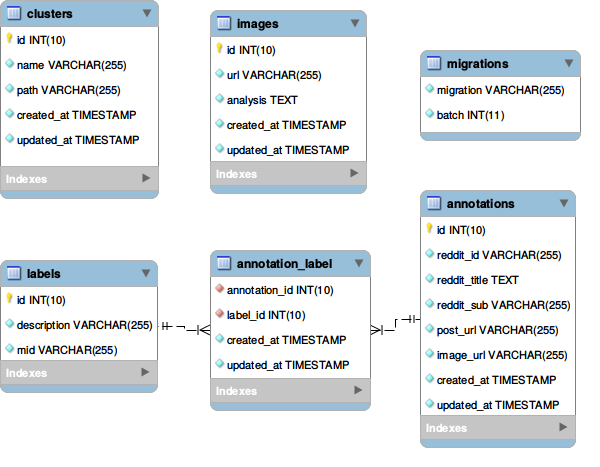
\includegraphics[width=\textwidth]{mysql_er_April_2.png}
\caption[MySQL Database schema]{
An ER diagram representing the MySQL database schema.}
\end{figure}

\subsection{BigQuery}
Querying massive datasets can not only be time consuming but expensive without the right hardware, infrastructure and software. \textit{Google} alleviates this problem with \textit{BigQuery}, an incredibly fast cloud-based storage platform. It is infrastructure as a service (IaaS) that handles all the hard work of both creating and accessing large data sets. Using the processing power of \textit{Google}, a user can get up and running with \textit{BigQuery} in a matter of minutes. The service can be used via their web UI, command-line tool or the REST API using one of the many client libraries. 
\par
Five months ago, user /u/Stuck{\_}In{\_}the{\_}Matrix of reddit collected all Reddit submission data from 2006 to 2015. He had effectively bundled 200 million submission objects, each with score data, author, title, self{\_}text, media tags and all the other attributes that are normally available via the Reddit API. The dataset complemented the Reddit comment corpus he released a couple months prior. When the data was initially made publicly available, he released it as a torrent where developers interested in using it could download their own local copies. Developers were all downloading the data for use either on their local machines or a cloud server. The problem with this is even with one of the most powerful desktop computers, loading the entire dataset into RAM was not feasible. Search times and joining (cross table) operations were expensive. 
\par
Conveniently soon after the release of this torrent, one of the lead engineers of \textit{Google BigQuery}, Felipe Hoffa, uploaded the data to \textit{BigQuery} and made the dataset publicly available. Each month, the dataset is updated with the latest information collected from the Reddit API.
\par
With the convenience of BigQuery, it is now possible to query gigabytes of history Reddit data in a matter of seconds. Listed below are a few of the integral queries used in \textit{Rally}, their sizes and the execution time.

% Best time to post on Reddit
\begin{figure}[!htb]
\begin{lstlisting}
SELECT subreddit, total, sub_hour, num_gte_3000
FROM (
	SELECT
		HOUR(SEC_TO_TIMESTAMP(created - 60*60*5)) as sub_hour,
		SUM(score >= 3000) as num_gte_3000,
		SUM(num_gte_3000) OVER(PARTITION BY subreddit) total, subreddit,
	FROM [fh-bigquery:reddit_posts.full_corpus_201509]
	WHERE YEAR(SEC_TO_TIMESTAMP(created))=2015
	GROUP BY sub_hour, subreddit
	ORDER BY subreddit, sub_hour
)
WHERE total>700
ORDER BY total DESC, sub_hour
\end{lstlisting}
\caption[Query finding the best hours to post on Reddit]{
The BigQuery SQL for finding the best hours to post on Reddit. This query processes 5.00GB across one table in roughly 8 seconds (~1.5 seconds when cached)}
\end{figure}

% Activity on Reddit over time
\begin{figure}[!htb]
\begin{lstlisting}
SELECT RIGHT('0'+STRING(peak),2)+'-'+subreddit, hour, c 
FROM (
  SELECT subreddit, hour, c, MIN(IF(rank=1,hour,null)) 
  OVER(PARTITION BY subreddit) peak 
  FROM (
    SELECT subreddit, HOUR(SEC_TO_TIMESTAMP(created_utc)) hour, COUNT(*) c, ROW_NUMBER() 
    OVER(PARTITION BY subreddit ORDER BY c ) rank 
    FROM [fh-bigquery:reddit_comments.2015_08] 
    WHERE subreddit IN (%subreddits) 
    AND score>2 
    GROUP BY 1, 2 )
    )
ORDER BY 1,2
\end{lstlisting}
\caption[Query finding the best hours to post on Reddit]{
Viewing activity (number of submissions) on subreddits over time. The wildcard \textit{\%subreddits} is replaced with a string comma-separated list of subreddits. This query processes 1.49GB across one table in roughly 2.5 seconds (~1.1 seconds when cached)}
\end{figure}

\subsubsection{Facades in Laravel with Google Services}
In web programming, quite often developers will need access to static references to classes. Facades provide a static interface to such classes that are available in the application's service container. By default Laravel ships with several facades. These static proxies to underlying classes in the service container provide the benefit of a terse, expressive syntax while maintaining more testability and flexibility than traditional static methods.
\par
The facade class itself only needs to implement a single method \textit{getFacadeAccessor}. It is that method's job to define what to resolve from the container. Behind the scenes, the base facade class (which all facades must extend) makes use of a magic-method, \textit{\_\_callStatic()}, which defers calls from the facade to the resolved object. 

% Registering the service provider
\begin{figure}[!htb]
\begin{lstlisting}
public function register()
{
	$this->app->bind('google', function () {
		$client = new Google_Client();
		$client->useApplicationDefaultCredentials();
		$client->addScope(Google_Service_Bigquery::BIGQUERY);
		
		return new GoogleAPI($client);
	});
}
\end{lstlisting}
\caption[Registering the Google service provider]{
Registering the Google service provider and binding the facade keyworld \textit{Google} to it.}
\end{figure}

The point of registering a facade may at times seem convoluted and unnecessary. It has always been a topic of discussion amongst the PHP world and a lot of the time boils down to personal preference and code readability. The facade approach was chosen particularly for \textit{BigQuery} part of the project for a few main reasons:
\begin{itemize}
  \item Expressive syntax without sacrificing testability of code
  \item Keep class responsibility narrow and well defined
  \item Clean constructor injection to automatically connect to \textit{Google Services} and access the \textit{BigQuery API}
  \item Explicit declaration defines what the class needs and what the class does
\end{itemize}

\section{phpRaw}
The Reddit API has several endpoints. It is through these endpoints where a client can retrieve posts specific to a subreddit, post a comment, moderate their account and all other actions that are normally available through the consumable web interface. For a single use or specific focus, calling the endpoints explicitly with cURL (or another client-side URL transfer) works fine but this strategy quickly fails as needs grow. Due to the wide array of endpoint calls utilized, it was necessary to develop an API wrapper that allows convenient calls to the API. Such a wrapper already existed for Python, Java, C and a few other languages but not PHP.
\par
An open source wrapper was discovered on GitHub but was no longer maintained, was not written to comply with the latest API security requirements (OAuth2) and was missing nearly half of the endpoints. Building on the work done on this API wrapper, a successful implementation was built and is what \textit{Rally} utilizes and depends on for direct Reddit data access. The GitHub repository from the point at which it was forked and built on is linked in the appendix.
\par 
Listed below are a functions from \textit{phpRaw} to give a feel for the wrapper.
% Get the user submitted data
\begin{center}
Get the user submitted data.
\end{center}
\begin{lstlisting}
$phpRaw->getUserSubmitted($user, $limit = 25, $after = null);
\end{lstlisting}

% Get the top 10 hottest listings for a specified subreddit
\begin{center}
Get the top 10 hottest listings for a specified subreddit.
\end{center}
\begin{lstlisting}
$phpRaw->getHot('funny', 10);
\end{lstlisting}
\par
\textit{phpRaw} was then modified to serve as a standalone vendor service brought in through Laravel's default dependency manager \textit{Composer}. By extracting the wrapper to a separate module, updating and maintaining the endpoints is simple as they are changed over time. Using the power of composer and package dependencies, by including the declaration as outlined in Figure \ref{fig:composer}, whenever composer is updated it automatically updates to the latest version of \textit{phpRaw}.

% Composer.json for phpRaw
\begin{figure}[!htb]
\begin{lstlisting}
...
"repositories": [
	{
		"name": "kevin/phpRAW",
		"type": "vcs",
		"url": "https://github.com/kevineger/phpRAW"
	}
],
...
\end{lstlisting}
\caption[Requiring phpRaw as a dependency in composer.]{
Requiring \textit{phpRaw} as a dependency for \textit{rally} in composer.}
\label{fig:composer}
\end{figure}


\newpage %newpage needed otherwise pagestyle applied to previous chapter. Does not actually create a new page
\pagestyle{fancy}\chead{Bibliography}\rhead{}\cfoot{}\rfoot{\thepage}
\bibliographystyle{ubco}
\bibliography{thesis_references}%name of your .bib file

\end{document}
\endinput